\documentclass[11pt]{article}
\usepackage{icmlko}
\begin{document}

\title{내가 방금 쓴 문장과 방금 쓴 코드를 검사했다 --- 한쪽은 살고 한쪽은 죽었다}
\author{월드모델 실험실}
\date{노트 383 · 2026년 8월 1일}
\maketitle

\begin{abstract}
노트 382에서 웹툰을 두고 ``수집이 요일별 연재작 전부 $+$ 완결 아카이브라
\emph{사실상 전수조사}이고, 최소 19는 우리가 자른 게 아니라 플랫폼의
성질에 가깝다''고 썼다. 무게 711로 판에서 제일 무거운 도메인에 대한
문장인데 \textbf{코드를 세어 보지 않고 읽기만 하고 썼다.} 세어 봤다.

\textbf{``전수조사''는 틀렸다.} 완결 아카이브는 69쪽 3,077건인데
\texttt{webtoon\_domain.title\_ids} 가 \texttt{range(1, 60)} 으로 돈다 ---
422건에 아예 못 닿는다. 게다가 \texttt{if len(fin) >= half: break} 가
1\,--\,59쪽 안에서도 543건을 더 남긴다. 연재작 45건까지 합쳐
\textbf{플랫폼 3,827건 중 우리는 2,817건, 74\%다.}

\textbf{그런데 결론은 살았다.} 빠진 1,010건에서 씨앗 고정으로 220건을
뽑아 관심 등록 수를 받아 보니 중앙이 \textbf{53,366} 으로 우리
\textbf{55,208} 과 사실상 같고(단측 MWU $p=0.045$), 최소가 \textbf{90} 으로
우리 최소 \textbf{19} 보다 오히려 높다. \textbf{우리 바닥 아래에 있는
빠진 작품이 0/220 이다.} 26\%를 못 받은 것은 덮음의 손해지 \emph{위를
떴다}는 뜻이 아니고, \textbf{바닥 19는 플랫폼의 것이 맞다.}

\textbf{그리고 같은 검사를 내 코드에 돌렸더니 죽었다.} 노트 382가 남의
수집이 목록 위를 뜬다고 지적하면서 새로 쓴
\texttt{ingest/game\_sample.py} 의 첫 31건이 \textbf{전부 오프셋 2,900
--- 목록 167,368건의 위 1.7\%} 에서 나왔다. 쪽을 오름차순으로 훑고 그
순서대로 상세를 받으니, 중간에 본 부분 결과가 목록 앞쪽만 담는다.
\textbf{``위를 떴다''고 쓰는 노트의 표본기가 위를 뜨고 있었다.} 씨앗으로
섞도록 고쳤다.
\end{abstract}

\section{문장 검사 --- 웹툰}

노트 382는 웹툰 수집 코드를 \emph{읽고} 엔드포인트가 인기순이 아니라는
것만 확인한 뒤 ``사실상 전수조사''라고 썼다. 플랫폼이 실제로 몇 건인지는
안 세었다. 세어 보니:

\begin{center}
\begin{tabular}{lrl}
\hline
 & 작품 수 & \\
\hline
우리 & 2,817 & \\
빠진 것: 완결 1\,--\,59쪽 & 543 & \texttt{len(fin) >= half} 조기 중단 \\
빠진 것: 완결 60쪽$+$ & 422 & \texttt{range(1, 60)} 이 못 닿는다 \\
빠진 것: 연재 & 45 & \\
\hline
플랫폼 전체 & 3,827 & 우리 몫 \textbf{74\%} \\
\hline
\end{tabular}
\end{center}

\textbf{빠진 것이 아래쪽인가.} 1,010건에서 220건을 씨앗 고정으로 뽑아
\texttt{article/list/info} 로 관심 등록 수를 받았다.

\begin{center}
\begin{tabular}{lrrr}
\hline
 & 행 & 중앙(관심 수) & 최소 \\
\hline
우리 & 2,817 & 55,208 & \textbf{19} \\
빠진 것 표본 & 220 & 53,366 & \textbf{90} \\
\hline
\end{tabular}
\end{center}

단측 MWU가 $p=0.045$ 로 빠진 쪽이 아주 조금 낮지만 중앙 차이가 3\%다.
\textbf{우리 최소 19 아래에 있는 빠진 작품은 0/220 이고, 우리 1분위(474)
아래도 9/220(4\%)뿐이다.} 조각별로는 \texttt{range(1,60)} 이 놓친 60쪽$+$가
중앙 30,373 으로 조금 낮고 1\,--\,59쪽은 66,184 로 오히려 높다.

\textbf{읽는 법: 웹툰은 덮음이 74\%지 위를 뜬 표본이 아니다.} 노트 382의
표에서 웹툰이 ``바닥 19 · census''로 분류된 것은 유지하되, ``전수조사''라는
말은 ``74\%이고 빠진 것이 같은 분포''로 고친다. \textbf{판에서 제일 무거운
도메인이 펀딩·게임과 같은 병은 아니다.}

\begin{figure}[t]
\centering
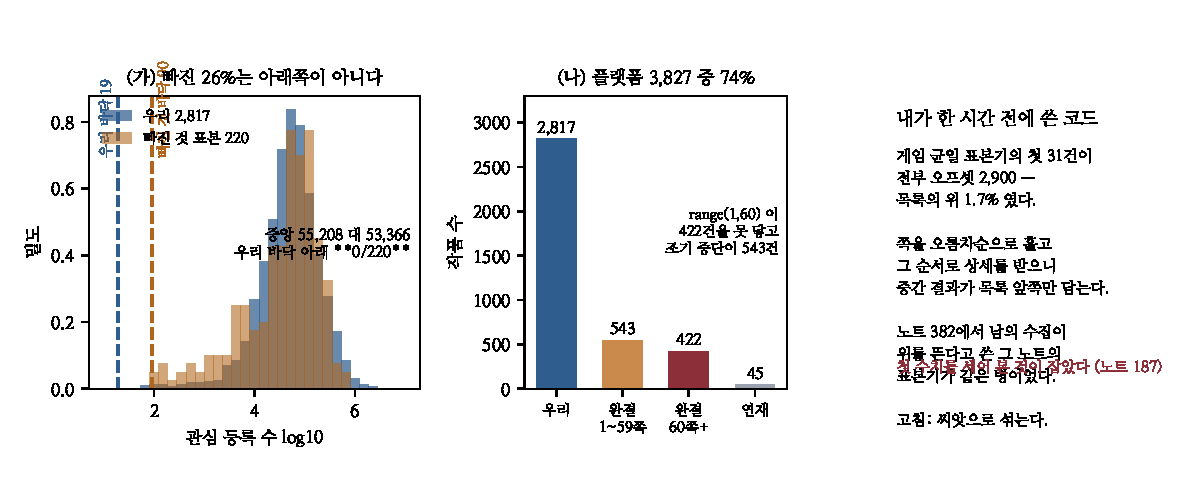
\includegraphics[width=\linewidth]{figs/fig383.pdf}
\caption{\textbf{(가)} 우리 2,817건과 빠진 것 표본 220건의 관심 등록 수
분포. 겹친다 --- 빠진 쪽 바닥(90)이 우리 바닥(19)보다 높다.
\textbf{(나)} 플랫폼 3,827건의 내역. \textbf{(다)} 같은 검사를 내 코드에
돌린 결과.}
\label{fig:main}
\end{figure}

\section{코드 검사 --- 내 것}

노트 382와 함께 \texttt{ingest/game\_sample.py} 를 새로 썼다. 목록
167,368건에서 씨앗 고정으로 오프셋을 뽑아 균일 표본을 만드는 코드다.
돌려 놓고 노트 187의 제일 싼 검사 --- \textbf{새 코드의 첫 수치는 세어
본다} --- 를 했다.

\begin{center}
\begin{tabular}{lr}
\hline
첫 31건의 오프셋 & \textbf{전부 2,900} \\
그 오프셋의 위치 & 167,368건 중 \textbf{위 1.7\%} \\
\hline
\end{tabular}
\end{center}

\texttt{sample\_ids} 가 오프셋을 \emph{정렬해서} 훑고 그 순서 그대로
\texttt{ids} 를 돌려주므로, 상세 받기가 오프셋 오름차순으로 돈다. 표본
전체를 다 받으면 균일하지만 \textbf{중간에 본 부분 결과는 목록 앞쪽만
담는다.} 그리고 이 수집은 몇 시간짜리라 부분 결과를 볼 수밖에 없다.

\textbf{남의 수집이 목록 위를 뜬다고 지적하는 노트의 표본기가 목록 위를
뜨고 있었다.} 고침은 한 줄이다 --- 씨앗으로 섞은 뒤 돌려준다
(\texttt{random.Random(SEED+1).shuffle(ids)}). 씨앗이 고정이라 재현된다.

\textbf{규약에 붙인다: 새로 쓴 수집기의 첫 수치는 라벨이 아니라 \emph{어디서
왔는지}를 센다.} 노트 271이 ``새 코드의 첫 수치는 행 수를 세어 본다''를
남겼는데, 수집기에서는 행 수가 아니라 \textbf{출처 좌표}(쪽 · 오프셋 ·
날짜)의 분포를 세야 한다. 행 수는 31로 맞았고 틀린 것은 그 31이 어디서
왔느냐였다.

\section{두 검사의 값이 다르다}

문장 검사는 결론을 바꾸지 않았다(웹툰은 여전히 안전하다). 코드 검사는
\textbf{앞으로 나올 수치 전체}를 바꿀 뻔했다 --- 안 고쳤으면 게임 균일
표본이 사실은 위 2\%짜리 표본이었을 것이고, 노트 379가 펀딩에서 잰
``위를 뜨면 4.8배 부풀어 보인다''를 게임에서 그대로 재현하면서 그것이
발견이라고 썼을 것이다.

\textbf{내 것을 먼저 검사한다.} 남의 수집 편향을 세는 노트일수록 그렇다.

\section{남은 것}

\begin{center}
\begin{tabular}{lll}
\hline
항목 & 왜 값이 큰가 & 어떻게 \\
\hline
게임 균일 2,000 & 고친 표본기로 다시 돈다 & 수집 중 · 노트 379 절차 \\
웹툰 1,010 & 덮음 74\% $\to$ 100\% & 분포가 같으니 급하진 않다 \\
도서 목록 구조 & \texttt{item\_ids} 가 주간 베스트셀러다 & 목록 전체 크기부터 센다 \\
수집기 출처 좌표 검사 & 이번에 한 번 살았다 & 기존 수집기 아홉에 소급 \\
\hline
\end{tabular}
\end{center}

\end{document}
